\documentclass[12pt,a4paper]{article}
\usepackage{amsmath,amscd,amsbsy,amssymb,latexsym,url,bm,amsthm}
\usepackage{epsfig,graphicx,subfigure}
\usepackage{enumitem,balance}
\usepackage{wrapfig}
\usepackage{mathrsfs,euscript}
\usepackage[usenames]{xcolor}
\usepackage{hyperref}
\usepackage{float}
\usepackage[vlined,ruled,linesnumbered]{algorithm2e}
\usepackage{array}
\hypersetup{colorlinks=true,linkcolor=black}
\usepackage{attachfile}
\usepackage{listings}

\newtheorem{theorem}{Theorem}
\newtheorem{lemma}[theorem]{Lemma}
\newtheorem{proposition}[theorem]{Proposition}
\newtheorem{corollary}[theorem]{Corollary}
\newtheorem{exercise}{Exercise}
\newtheorem*{solution}{Solution}
\newtheorem{definition}{Definition}
\theoremstyle{definition}

\renewcommand{\thefootnote}{\fnsymbol{footnote}}

\newcommand{\postscript}[2]
 {\setlength{\epsfxsize}{#2\hsize}
  \centerline{\epsfbox{#1}}}

\renewcommand{\baselinestretch}{1.0}

\setlength{\oddsidemargin}{-0.365in}
\setlength{\evensidemargin}{-0.365in}
\setlength{\topmargin}{-0.3in}
\setlength{\headheight}{0in}
\setlength{\headsep}{0in}
\setlength{\textheight}{10.1in}
\setlength{\textwidth}{7in}
\makeatletter \renewenvironment{proof}[1][Proof] {\par\pushQED{\qed}\normalfont\topsep6\p@\@plus6\p@\relax\trivlist\item[\hskip\labelsep\bfseries#1\@addpunct{.}]\ignorespaces}{\popQED\endtrivlist\@endpefalse} \makeatother
\makeatletter
\renewenvironment{solution}[1][Solution] {\par\pushQED{\qed}\normalfont\topsep6\p@\@plus6\p@\relax\trivlist\item[\hskip\labelsep\bfseries#1\@addpunct{.}]\ignorespaces}{\popQED\endtrivlist\@endpefalse} \makeatother

\begin{document}
\noindent

%========================================================================
\noindent\framebox[\linewidth]{\shortstack[c]{
\Large{\textbf{Lab06-Linear Programming}}\vspace{1mm}\\
CS214-Algorithm and Complexity, Xiaofeng Gao, Spring 2021.}}
\begin{center}
\footnotesize{\color{red}$*$ If there is any problem, please contact TA Haolin Zhou.}

% Please write down your name, student id and email.
\footnotesize{\color{blue}$*$ Name:Yanjie Ze  \quad Student ID:519021910706 \quad Email: zeyanjie@sjtu.edu.cn}
\end{center}

\begin{enumerate}
    \item
    \textit{Hirschberg Algorithm.} Recall the \textbf{String Similarity} problem in class, in which we calculate the edit distance between two strings in a sequence alignment manner.
    \begin{enumerate}
    	\item
    	Implement the algorithm combining \textbf{dynamic programming} and \textbf{divide-and-conquer} strategy in C/C++. Analyze the time complexity of your algorithm. {\color{blue}(The template \emph{Code-SequenceAlignment.cpp} is attached on the course webpage)}.
    	\begin{solution}
    	~\\
    	In \textbf{Code-SequenceAlignment.cpp}, we use divide-and-conquer mixed with dynamic programming to solve the string similarity problem.
    	~\\
    	
    	We use the same denote as that in our class. Denote $f(i,j)$ as the shortest path from $(0,0)$ to $(i,j)$, $g(i,j)$ as the shortest path from $(i,j)$ to $(m,n)$. Then the cost of the shortest path using $(i,j)$ is $f(i,j)+g(i,j)$.
    	
    	Then, the main process of the algorithm is illustrated in Fig.~\ref{q1}.
        \begin{enumerate}
            \item First, we divide the region(a $m\times n$ matrix) into two part, each of which is $m\times \frac{n}{2}$.
            \item Next, we find the pivot$(q,\frac{n}{2})$ which minimizes $f(i,\frac n2) + g(i,\frac n2)$.
            \item Then we continue doing \textbf{Divide and DP} in the subregions, until we figure out all the pivot, consisting of the whole sequence-alignment path.
        \end{enumerate}
    	\begin{figure}[htbp]
    	    \centering
    	    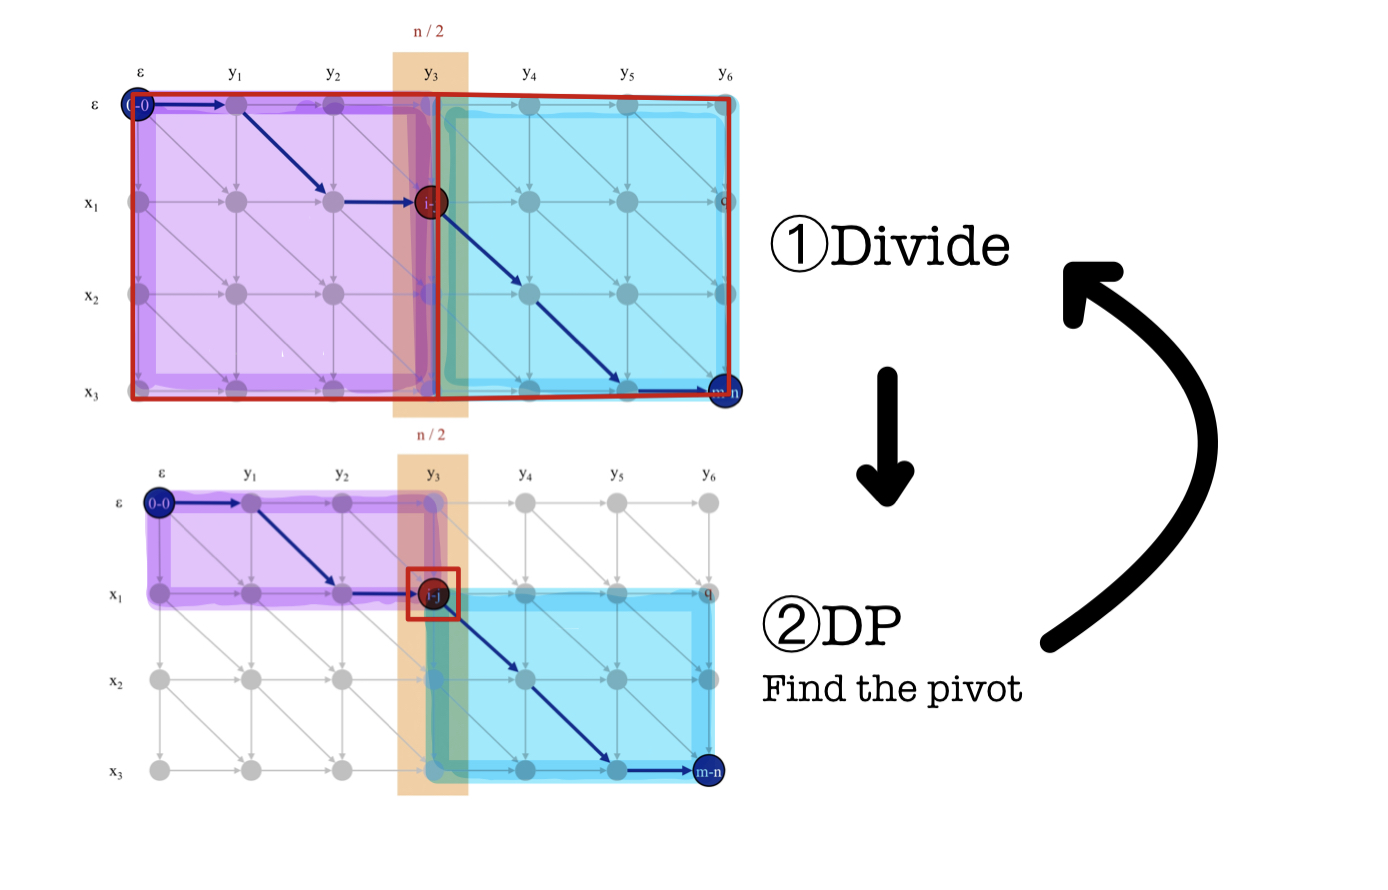
\includegraphics[width=10cm]{q1.jpg}
    	    \caption{Hirschberg Algorithm}
    	    \label{q1}
    	\end{figure}
    	
    	\textbf{Time complexity}: $O(mn)$
    	
    	To find a pivot in a $m\times n$ matrix, we need $O(mn)$ time based on tabular dynamic programming.Denote $pivot(m,n)=O(mn)$.
    	
        Assume the region area is described as $(x_{low}, y_{low}, x_{high}, y_{high})$, representing the four corners. After finding a pivot$(i,j)$ in this region$(x_{low}, y_{low}, x_{high}, y_{high})$, the region is divided into two subregions: $(x_{low}, y_{low}, i, j)$, and $(i, j, x_{high}, y_{high})$. 
        
        Finally, we have the equation:

    	$$
    	T(m,n) = T(q,\frac n2) + T(m-q,\frac n2) + pivot(m,n) = O(m,n)
    	$$
    	
        In our class ,we have used \textbf{mathematical induction} to prove $T(m,n) = O(m,n)$ with this equation, so we will not give unnecessary details.
    	\end{solution}
    	\item
    	Given $\alpha(x, y) = |ascii(x) - acsii(y)|$, where $ascii(c)$ is the ASCII code of character $c$, and $\delta=13$. Find the edit distance between the following two strings.
    	\begin{align*}
    		X[1..60]=&\ CMQHZZRIQOQJOCFPRWOUXXCEMYSWUJ\\
    		&\ TAQBKAJIETSJPWUPMZLNLOMOZNLTLQ	
    	\end{align*}
    	\begin{align*}
    		Y[1..50]=&\ SUYLVMUSDROFBXUDCOHAATBKN\\
    		&\ AAENXEVWNLMYUQRPEOCJOCIMZ
    	\end{align*}
    	\begin{solution}
    	The edit distance between the two strings is $385$, as Fig~\ref{output} shows.
    	\begin{figure}[htbp]
    	    \centering
    	    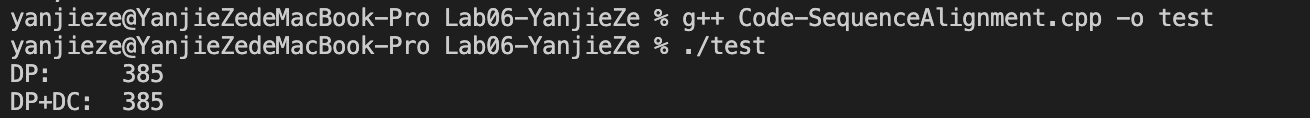
\includegraphics[width=10cm]{q1result.png}
    	    \caption{Program Output for Hirschberg Algorithm}
    	    \label{output}
    	\end{figure}
    	\end{solution}
    \end{enumerate}
    
    
    \item 
    \textit{Travelling Salesman Problem.} Given a list of cities and the distances between each pair of cities ($ G=(V,E,W) $), we want to find the shortest possible route that visits each city exactly once and returns to the origin city. Similar to \textbf{Maximum Independent Set} and \textbf{Dominating Set}, please turn the traveling salesman problem into an ILP form.  
    
    \textbf{Remark:} $ W $ is the set of weights corresponds to the edges that connecting adjacent cities.  
    
    \begin{solution}
    ~\\
    Denote the cities as $\{1,2,...,n\}$.Denote the distance between two cities $i,j$ is $w_{ij}$.
    
    
    Define:
    $$ 
			x_{ij}=\left\{
            \begin{aligned}
            & 1, if\ the\ path\ goes\ from\ city\ i\ to\ city\ j \\
            & 0, otherwsie
            \end{aligned}
            \right.
            $$
    Then we can formulate TSP problem into integer linear programming problem:
    $$
    \displaystyle \min \sum_{i=1}^n\sum_{j\neq i,j=1}^n w_{ij}x_{ij}
    $$
    $$
    s.t.\left\{
    \begin{aligned}
    & \sum_{i=1,i\neq j}^n x_{ij} = 1, &j=1,2,...,n\\
    & \sum_{j=1,j\neq i}^n x_{ij} = 1,  &i=1,2,...,n\\
    & \sum_{i\in Q}\sum_{j\neq i,j\in Q}x_{ij}\leq |Q|-1,  \quad &\forall Q \subseteq \{1,2,...,n\},|Q|\geq 2 
    \end{aligned}
    \right.
    $$
    \textbf{Explanation:}
    \begin{itemize}
        \item The first constraint means each city is arrived from exactly one other city.
        \item The second constraint means each city is departed from exactly one other city.
        \item The third constraint means the final tour can't be the union of small subtours, as illustrated in Fig.~\ref{tour}. If the tour consists of subtours, as shown in Fig.~\ref{tour}(1), then $\sum_{i\in Q}\sum_{j\neq i,j\in Q}x_{ij}\geq |Q|$. Otherwise, $\sum_{i\in Q}\sum_{j\neq i,j\in Q}x_{ij}\leq |Q|-1$, shown in Fig.~\ref{tour}(2).
        
    \end{itemize}
    This formulation is also called \textbf{Dantzig–Fulkerson–Johnson formulation}. Other common formulations, such as \textbf{Miller–Tucker–Zemlin formulation}, will not be introduced here.
    \begin{figure}[htbp]
        \centering
        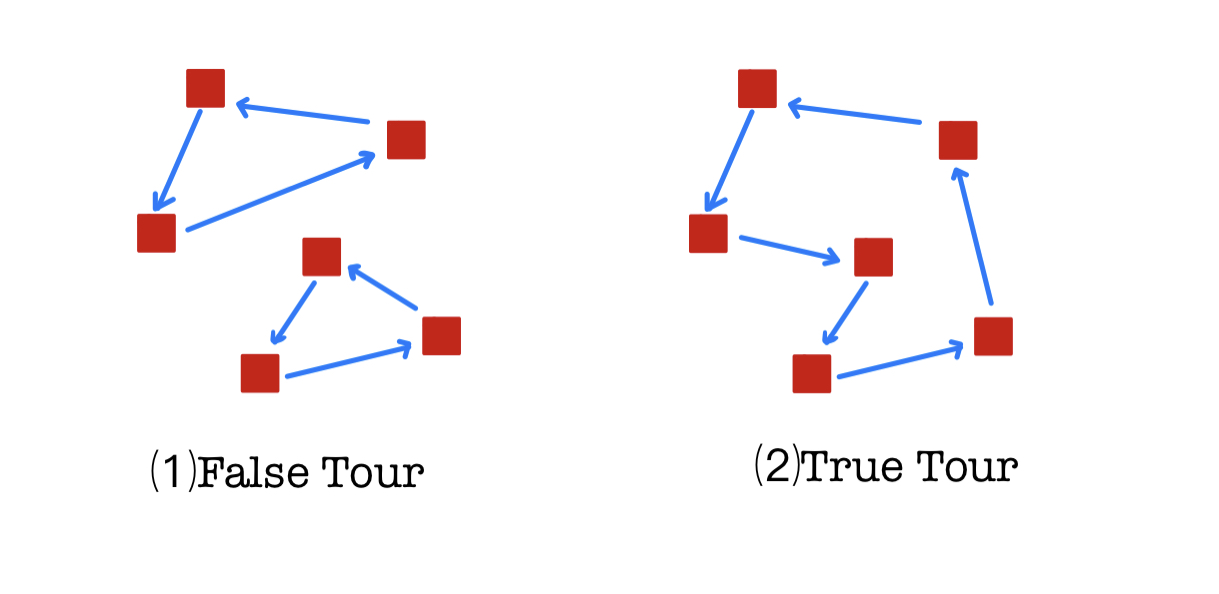
\includegraphics[width=10cm]{tour.jpg}
        \caption{Explanation of Constraint 3 in TSP}
        \label{tour}
    \end{figure}
    \end{solution}
    \item
    \textit{Investment Strategy.} A company intends to invest $0.3$ million yuan in $2021$, with a proper combination of the following $3$ projects:
    \begin{itemize}
    \item \textbf{Project 1:} Invest at the beginning of a year, and can receive a $20\%$ profit of the investment in this project at the end of this year. Both the capital and profit can be invested at the beginning of next year;
    \item \textbf{Project 2:} Invest at the beginning of $2021$, and can receive a $50\%$ profit of the investment in this project at the end of $2022$. The investment in this project cannot exceed $0.15$ million dollars;
    \item \textbf{Project 3:} Invest at the beginning of $2022$, and can receive a $40\%$ profit of the investment in this project at the end of $2022$. The investment in this project cannot exceed $0.1$ million dollars.
    \end{itemize}
    Assume that the company will invest \emph{all} its money at the beginning of a year. Please design a scheme of investment in $2021$ and $2022$ which maximizes the overall sum of capital and profit at the end of $2022$.
    \begin{enumerate}
    \item
    Formulate a linear programming with necessary explanations.
    \begin{solution}
    Based on the problem description we denote five variables, listed in Table~\ref{table1}.
    \begin{center}
    \begin{tabular}{|c|c|}
    \hline
    \multicolumn{2}{|c|}{Variable Denote}\\
        \hline
        \label{table1}
      $x_1$   &  the capital invested in project 1 in 2021\\
      \hline
      $x_2$   &  the capital invested in project 2 in 2021\\
      \hline
      $x_3$   &  the capital invested in project 1 in 2022\\
      \hline
      $x_4$   &  the capital invested in project 3 in 2022 \\
      \hline
   
    \end{tabular}
    \end{center}
     Four basic constraints:
     $$
     x_1\geq 0
     $$
    $$
    0\leq x_2 \leq 0.15
    $$
    $$
    x_3 \geq 0
    $$
    $$
    0\leq x_4 \leq 0.1
    $$
    In the first year(2021), we have 0.3 million and invest all:
    $$
    x_1 + x_2 = 0.3
    $$
    Then in the next year(2022), we use the capital and profit to invest again:
    $$
    x_3 + x_4 = 1.2x_1
    $$
    At the end of 2022, the capital and profit sums together:
    $$
    target = 1.5x_2 + 1.2x_3 + 1.4x_4
    $$
    Therefore, we have such linear programming formulation:
    $$
    \max 1.5x_2 + 1.2x_3 + 1.4x_4
    $$
    
    $$
    s.t.\left\{
    \begin{aligned}
    &x_1 + x_2 = 0.3\\
    &x_3 + x_4 = 1.2x_1\\
    &x_1\geq 0\\
    &0\leq x_2 \leq 0.15\\
    &x_3 \geq 0\\
    &0\leq x_4 \leq 0.1
    \end{aligned}
    \right.
    $$
    \end{solution}
    \item
    Transform your LP into its standard form and slack form.
    \begin{solution}
    ~\\
    \textbf{Standard Form:}
    $$
    \max 1.5x_2 + 1.2x_3 + 1.4x_4
    $$
    
    $$
    s.t.\left\{
    \begin{aligned}
    &x_1 + x_2 \leq 0.3\\
    &-x_1 - x_2 \leq -0.3\\
    &x_3 + x_4 - 1.2x_1\leq 0\\
    &-x_3 - x_4 + 1.2x_1\leq 0\\
    &x_2 \leq 0.15\\
    &x_4 \leq 0.1\\
    &x_1,x_2,x_3,x_4\geq 0
    \end{aligned}
    \right.
    $$
    
    \textbf{Slack Form: }
    $$
    \max 1.5x_2 + 1.2x_3 + 1.4x_4
    $$
    
    $$
    s.t.\left\{
    \begin{aligned}
    &x_1 + x_2+x_5 = 0.3\\
    &-x_1 - x_2 + x_6 = -0.3\\
    &x_3 + x_4 - 1.2x_1 + x_7 =  0\\
    &-x_3 - x_4 + 1.2x_1+x_8= 0\\
    &x_2 +x_9 =  0.15\\
    &x_4 +x_{10}=  0.1\\
    &x_1,x_2,x_3,x_4,x_5,x_6,x_7,x_8,x_9,x_{10}\geq 0
    \end{aligned}
    \right.
    $$
    
    \end{solution}
    \item
    Transform your LP into its dual form.
    \begin{solution}
    ~\\
    \begin{center}
        \begin{tabular}{c c}
        \hline
           Multiplier & Constraint \\
           \hline
            $y_1$  &$x_1 + x_2 \leq 0.3$\\
           $y_2$ &$-x_1 - x_2 \leq -0.3$\\
          $y_3$  &$x_3 + x_4 - 1.2x_1\leq 0$\\
            $y_4$ &$-x_3 - x_4 + 1.2x_1\leq 0$\\
           $y_5$ &$x_2 \leq 0.15$\\
           $y_6$ &$x_4 \leq 0.1$\\
           \hline
        \end{tabular}
    \end{center}
    $$
    (y_1-y_2-1.2y_3+1.2y_4)x_1 + (y_1-y_2+y_5)x_2 + (y_3-y_4)x_3 + (y_3-y_4+y_6)x_4 
    $$
    $$
    \leq 0.3y_1 -0.3y_2 + 0.15y_5 + 0.1y_6
    $$
    Then:
    $$
    1.5x_2 + 1.2x_3 + 1.4x_4 \leq 0.3y_1 -0.3y_2 + 0.15y_5 + 0.1y_6
    $$
    So \textbf{the dual form} is:
    $$
    \min 0.3y_1 -0.3y_2 + 0.15y_5 + 0.1y_6
    $$
    $$
    s.t.\left\{
    \begin{aligned}
    &y_1,y_2,y_3,y_4,y_5,y_6 \geq 0 \\
    &y_1-y_2-1.2y_3+1.2y_4 \geq 0 \\
    &y_1-y_2+y_5 \geq 1.5\\
    &y_3-y_4 \geq 1.2\\
    &y_3-y_4+y_6 \geq 1.4\\
    \end{aligned}
    \right.
    $$
    \end{solution}
    
    
    \item
    Use the simplex method to solve your LP.
    \begin{solution}
    ~\\
    We simplify \textbf{Slack Form} before:
    $$
    \max 1.5x_2 + 1.2x_3 + 1.4x_4
    $$
    
    $$
    s.t.\left\{
    \begin{aligned}
    &x_1 + x_2 = 0.3\\
    &x_3 + x_4 - 1.2x_1 =  0\\
    &x_2 +x_5 =  0.15\\
    &x_4 +x_{6}=  0.1\\
    &x_1,x_2,x_3,x_4,x_5,x_{6}\geq 0
    \end{aligned}
    \right.
    $$
    
    One basic solution: $x_1=0.3,x_2=0,x_3=0.36,x_4=0,x_5=0.15,x_6=0.1$.
    
    Then we use simplex method:
    \begin{enumerate}
        \item Select $x_2$, which is bounded by $x_2=0.3-x_1$ and $x_2 = 0.15 - x_5$. So replace $x_2$ with $0.15-x_5$. 
        
        Then the solution: $\hat{x}=\{0.15,0.15,0.36,0,0,0.1\}$.
        
        The target: $ 0.225-1.5x_5 + 1.2x_3 + 1.4x_4$.
        \item Select $x_4$, which is bounded by $x_4 = 0.1 - x_6$ and $x_4 = 1.2x_1-x_3=0.18-x_3$. Replace $x_4$ with $0.1-x_6$. 
        
        Then the solution: $\hat{x}=\{0.15,0.15,0.08,0.1,0,0\}$
        
        The target: $0.225-1.5x_5 + 1.2x_3 + 0.14- 1.4x_6$
        \item Prove such solution is optimal. If we still want to improve $x_3$, we have :
        $$x_3=1.2x_1-x_4=0.36-1.2x_2-x_4$$.
        
        Thus:
        $$\Delta x_3 = -1.2\Delta x_2 - \Delta x_4$$
        However, in out target: 
        $$
        \Delta target = 1.5\Delta x_2 + 1.2\Delta x_3 + 1.4\Delta x_4
        $$
        
        Which means either sacrificing $x_2$ or $x_4$ to improve $x_3$ will not improve the target further, when $x_2$ and $x_4$ have reaching the limit.
        
        Therefore, the solution $\hat{x}=\{0.15,0.15,0.08,0.1,0,0\}$ is optimal.
        
    \end{enumerate}
    Finally, we get $\mathbf{x_1 = 0.15, x_2=0.15,x_3=0.08,x_4=0.1}$, and the maximum sum of capital and profit is $\mathbf{0.461}$ million.
    \end{solution}
    \end{enumerate}
    \item
    \textit{Factory Production.} An engineering factory makes seven products (PROD 1 to PROD 7) on the following machines: four grinders, two vertical drills, three horizontal drills, one borer and one planer. Each product yields a certain contribution to profit (in \pounds/unit). These quantities (in \pounds/unit) together with the unit production times (hours) required on each process are given below. A dash indicates that a product does not require a process.

    \begin{table}[htbp]
      \scriptsize
      \centering
      \renewcommand\arraystretch{1.1}
      \begin{tabular}{m{0.18\textwidth} m{0.07\textwidth}<{\centering} m{0.07\textwidth}<{\centering} m{0.07\textwidth}<{\centering} m{0.07\textwidth}<{\centering} m{0.07\textwidth}<{\centering} m{0.07\textwidth}<{\centering} m{0.07\textwidth}<{\centering}}
      \hline
       & \textbf{PROD 1} & \textbf{PROD 2} & \textbf{PROD 3} & \textbf{PROD 4} & \textbf{PROD 5} & \textbf{PROD 6} &  \textbf{PROD 7} \\\hline
      Contribution to profit & 10 & 6 & 8 & 4 & 11 & 9 & 3 \\
      Grinding & 0.5 & 0.7 & - & - & 0.3 & 0.2 & 0.5 \\
      Vertical drilling & 0.1 & 0.2 & - & 0.3 & - & 0.6 & - \\
      Horizontal drilling & 0.2 & - & 0.8 & - & - & - & 0.6 \\
      Boring & 0.05 & 0.03 & - & 0.07 & 0.1 & - & 0.08 \\
      Planing & - & - & 0.01 & - & 0.05 & - & 0.05 \\
      \hline
      \end{tabular}
    \end{table}

    There are marketing limitations on each product in each month, given in the following table:

    \begin{table}[htbp]
      \scriptsize
      \centering
      \renewcommand\arraystretch{1.1}
      \begin{tabular}{m{0.1\textwidth} m{0.07\textwidth}<{\centering} m{0.07\textwidth}<{\centering} m{0.07\textwidth}<{\centering} m{0.07\textwidth}<{\centering} m{0.07\textwidth}<{\centering} m{0.07\textwidth}<{\centering} m{0.07\textwidth}<{\centering}}
      \hline
       & \textbf{PROD 1} & \textbf{PROD 2} & \textbf{PROD 3} & \textbf{PROD 4} & \textbf{PROD 5} & \textbf{PROD 6} &  \textbf{PROD 7} \\\hline
      January & 500 & 1000 & 300 & 300 & 800 & 200 & 100 \\
      February & 600 & 500 & 200 & 0 & 400 & 300 & 150 \\
      March & 300 & 600 & 0 & 0 & 500 & 400 & 100 \\
      April & 200 & 300 & 400 & 500 & 200 & 0 & 100 \\
      May & 0 & 100 & 500 & 100 & 1000 & 300 & 0 \\
      June & 500 & 500 & 100 & 300 & 1100 & 500 & 60 \\
      \hline
      \end{tabular}
    \end{table}

    It is possible to store up to 100 of each product at a time at a cost of \pounds0.5 per unit per month (charged at the end of each month according to the amount held at that time). There are no stocks at present, but it is desired to have a stock of exactly 50 of each type of product at the end of June. The factory works six days a week with two shifts of 8h each day. It may be assumed that each month consists of only 24 working days. Each machine must be down for maintenance in one month of the six. No sequencing problems need to be considered.

    When and what should the factory make in order to maximize the total net profit?

    \begin{enumerate}
    \item
    Use \emph{CPLEX Optimization Studio} to solve this problem. Describe your model in \emph{Optimization Programming Language} (OPL). Remember to use a separate data file (.dat) rather than embedding the data into the model file (.mod).
    \begin{solution}
    ~\\
    First, we define some constants based on the problem description. Each constant has the meaning corresponding to its name, so we will not do further explanation. 
    
    
    \begin{center}

    \begin{tabular}{|c| c|}
    
    \hline
    number & meaning \\
    \hline
    \label{p4table}
       $1,2,3,4$ & four grinders\\
       $5,6$ & two vertical drills\\
       $7,8,9$ & three horizontal drills\\
       $10$ & one borer\\
       $11$ & one planer\\
       \hline
       
    \end{tabular}
            
    \end{center}
    
    \textbf{Notice}: we define the range $\mathbf{machine\_num}$ to represent all 11 machines, and we use the denote in table.~\ref{p4table} to number all the machines.
    
    	\lstset{
		language=C,
		tabsize=2,
		basicstyle=\footnotesize\ttfamily,
		columns=fullflexible,
		keywordstyle=\color{blue},
		numbers=left,
		numberstyle=\scriptsize\ttfamily,
		frame=single
	}
    \begin{lstlisting}
 {string} Prod=...;
 {string} Process = ...;
 float ProfitProd[Prod]=...;
 
 int NbMonths = ...;
 range month=1..NbMonths;
 float ProcessProd[Process][Prod]=...;
 int MarketProd[month][Prod]=...;
 
 float CostHold = ...;
 int StartHold = ...;
 int EndHold = ...;
 int MaxHold = ...;
 
 int HoursMonth = ...;
 int NumProcess[Process]=...;
 int NumDown[Process]=...;
 
 int machines = 4+2+3+1+1;
 range machine_num = 1..machines;
 
    \end{lstlisting}
    
Second, we define the decision variables mainly according to what we want to figure out, consisting of the months for maintenance, the amount of selling,making and holding. And we define the decision expressions similarly, as shown below.
\begin{lstlisting}
 dvar boolean maintenance[month][machine_num];
 dvar int+ product_make[month][Prod];
 dvar int+ product_sell[month][Prod];
 dvar int+ product_hold[month][Prod]; 
 
 dexpr float selling_profit = 
 sum(m in month) sum(p in Prod)product_sell[m][p]*ProfitProd[p];
 dexpr float holding_cost = 
 sum(m in month) sum(p in Prod) product_hold[m][p]*CostHold;
 dexpr float net_profit=selling_profit-holding_cost;
\end{lstlisting}

Third, we propose the constraints and the optimization target. The target is to maximize $net\_profit$. The constraints are separated into following parts: $maintain\_machine$, $basic\_hold\_calculation$, $final\_hold$, $make\_limit$,$store\_limit$, $sell\_limit$, and their meanings are listed in table~\ref{p4table2}.

\begin{center}
    \begin{tabular}{|c|c|}
    \hline
    \label{p4table2}
     Constraint    &  Meaning\\
     \hline
       $main\_machine$  & Each machine must be down in one month of six \\
       $basic\_hold\_calculation$ & Calculate the storage for each product in each month \\
       $final\_hold$ & Store exactly 50 of each type of product at the end of June \\
       $make\_limit$ & The limitation of making products caused by the machines \\
       $store\_limit$ & Store up to 100 of each product in each month \\
       $sell\_limit$ & The limitation of selling products because of the market\\
       \hline
    \end{tabular}
\end{center}

Then Optimization Programming Language is shown below.

\begin{lstlisting}
maximize net_profit;
 subject to
 {
 forall(machine in machine_num)
   maintain_machine:
   	sum(m in month)maintenance[m][machine] == 5;
forall(p in Prod){
  forall(m in month)
    basic_hold_calculation: 
    {if(m==1)
    product_hold[m][p] == product_make[m][p] - product_sell[m][p];
    else
    	product_hold[m][p] == product_hold[m-1][p] + product_make[m][p] - product_sell[m][p];}	
	final_hold: product_hold[6][p] == EndHold;	}
 forall(m in month){
   make_limit:{
   sum(p in Prod)product_make[m][p]*ProcessProd["Grind"][p] <= HoursMonth* (maintenance[m][1]+maintenance[m][4]+maintenance[m][2]+maintenance[m][3]);
   sum(p in Prod)product_make[m][p]*ProcessProd["VDrill"][p] <= HoursMonth* (maintenance[m][5]+maintenance[m][6]);
   sum(p in Prod)product_make[m][p]*ProcessProd["HDrill"][p] <= HoursMonth* (maintenance[m][7]+maintenance[m][8]+maintenance[m][9]);
   sum(p in Prod)product_make[m][p]*ProcessProd["Bore"][p] <= HoursMonth* (maintenance[m][10]);
   sum(p in Prod)product_make[m][p]*ProcessProd["Plane"][p] <= HoursMonth* (maintenance[m][11]);
 }   
 store_limit:
 	forall(p in Prod)product_hold[m][p] <= MaxHold; 
 sell_limit:
 	forall(p in Prod)product_sell[m][p] <= MarketProd[m][p];
}} 
\end{lstlisting}

    \end{solution}
    \item
    Solve your model and give the following results.
    \begin{enumerate}
    \item
    For each machine:
    \begin{enumerate}
    \item
    the month for maintenance.
    \end{enumerate}
    \item
    For each product:
    \begin{enumerate}
    \item
    The amount to make in each month.
    \item
    The amount to sell in each month.
    \item
    The amount to hold at the end of each month.
    \end{enumerate}
    \item
    The total selling profit.
    \item
    The total holding cost.
    \item
    The total net profit (selling profit minus holding cost).
    \end{enumerate}
    \end{enumerate}
    \textbf{Remark:} You can choose to use the attached .dat file or write it yourself. 
\begin{solution}
\begin{enumerate}
\item Solved before.
\item
\begin{enumerate}

    \item 
    The meaning of numbers has been explained before, in table~\ref{p4table}. 
    
    The maintenance condition is shown in table.~\ref{maint}, where $0$ means the machine is in maintenance and $1$ means the machine is in work.
    
    \begin{table}[htbp]
        \centering
        \begin{tabular}{|c|ccccccccccc|}
        \hline
         month$\backslash$ machine&1&	2&	3&	4	&5&	6&	7&	8&	9&	10&	11\\
         \hline
1&1&	1&	1&	1&	1&	1&	1&	1&	1&	1&	1\\
2&1&	1&	1&	0&	0&	1&	1&	1&	1&	1&	1\\
3&1&	1&	1&	1&	1&	1&	1&	1&	1&	1&	1\\
4&0&	1&	1&	1&	1&	1&	1&	1&	1&	0&	0\\
5&1&	0&	0&	1&	1&	0&	1&	0&	1&	1&	1\\
6&1&	1&	1&	1&	1&	1&	0&	1&	0&	1&	1\\
\hline

    \end{tabular}
        \caption{Months for Maintenance}
        \label{maint}
    \end{table}

\item
The amount to make in eahc month is shown in table~\ref{amount_make}.The amount to sell in each month is shown in table~\ref{amount_sell}.
The amount to hold in each month is shown in table.~\ref{amount_hold}.

\begin{table}[htbp]
    \centering
    \begin{tabular}{|c|ccccccc|}
    \hline
       month$\backslash$product & Prod1 &	Prod2&	Prod3 &	Prod4 &	Prod5&	Prod6&	Prod7\\
       \hline
1&500&	1000&	300	&300&	800	&200&	100\\
2&600&	500&	200	&0&	400&	300&	150\\
3&400&	700	&100&	100&	600	&400&	200\\
4&0&	0&	0&	0&	0& 0&	0\\
5&0	&100&	500&	100	&1000&	300&	0\\
6&550&	550&	150	&350&	1150&	550&	110\\
\hline
    \end{tabular}
    \caption{Amount to Make}
    \label{amount_make}
\end{table}

\begin{table}[htbp]
    \centering
    \begin{tabular}{|c|ccccccc|}
    \hline
        month$\backslash$product & Prod1 &	Prod2&	Prod3 &	Prod4 &	Prod5&	Prod6&	Prod7\\
        \hline
1&500&	1000&	300	&300&	800	&200&	100\\
2&600	&500&	200&	0&	400&	300&	150\\
3&300	&600&	0&	0&	500	&400&	100\\
4&100&	100&	100&	100&	100&	0&	100\\
5&0&	100	&500&	100&	1000&	300&	0\\
6&500&	500&	100	&300&	1100&	500&	60\\
\hline
    \end{tabular}
    \caption{Amount to Sell}
    \label{amount_sell}
\end{table}

\begin{table}[H]
    \centering
    \begin{tabular}{|c|ccccccc|}
    \hline
        month$\backslash$product & Prod1 &	Prod2&	Prod3 &	Prod4 &	Prod5&	Prod6&	Prod7\\
        \hline
 
1&0&	0&	0&	0&	0&	0&	0\\
2&0&	0&	0&	0&	0&	0&	0\\
3&100&	100	&100&	100&	100&	0&	100\\
4&0	&0&	0&	0&	0&	0&	0\\
5&0&	0&	0&	0&	0&	0&	0\\
6&50&	50&	50&	50&	50&	50&	50\\
\hline

    \end{tabular}
    \caption{Amount to Hold}
    \label{amount_hold}
\end{table}
\item The total selling profit is \textbf{109330}.
\item The total holding cost is \textbf{475}.
\item The total net profit is \textbf{108855}.

    \end{enumerate}
\end{enumerate}
\end{solution}
\end{enumerate}
\newpage
\vspace{20pt}

{\noindent\large\textbf{Appendix}}
\begin{enumerate}
	\item [\textbf{A.}]
	\textbf{FactoryPlanning.dat}
	\attachfile{FactoryPlanning.dat}
	\lstset{
		language=C,
		tabsize=2,
		basicstyle=\footnotesize\ttfamily,
		columns=fullflexible,
		keywordstyle=\color{blue},
		numbers=left,
		numberstyle=\scriptsize\ttfamily,
		frame=single
	}
	\begin{lstlisting}
		NbMonths = 6;
		
		Prod = {Prod1, Prod2, Prod3, Prod4, Prod5, Prod6, Prod7};
		Process = {Grind, VDrill, HDrill, Bore, Plane};
		
		// profitProd[j] is profit per unit for product j
		ProfitProd = [10 6 8 4 11 9 3];
		
		// processProd[i][j] gives hours of process i required by product j
		ProcessProd = [[0.5  0.7  0.0  0.0  0.3  0.2 0.5 ]
		[0.1  0.2  0.0  0.3  0.0  0.6 0.0 ]
		[0.2  0.0  0.8  0.0  0.0  0.0 0.6 ]
		[0.05 0.03 0.0  0.07 0.1  0.0 0.08]
		[0.0  0.0  0.01 0.0  0.05 0.0 0.05]];
		
		// marketProd[i][j] gives marketing limitation on product j for month i
		MarketProd = [[500 1000 300  300 800  200 100]
		[600 500  200  0   400  300 150]
		[300 600  0    0   500  400 100]
		[200 300  400  500 200  0   100]
		[0   100  500  100 1000 300 0  ]
		[500 500  100  300 1100 500 60 ]];
		
		CostHold  = 0.5;
		StartHold = 0;
		EndHold   = 50;
		MaxHold   = 100;
		
		// process capacity
		HoursMonth = 384; // 2 eight hour shifts per day, 24 working days per month;
		
		// number of each type of machine
		NumProcess = [4 2 3 1 1];
		
		// how many machines must be down over 6 month period
		NumDown = [4 2 3 1 1];
	\end{lstlisting}
\end{enumerate}

\textbf{Remark:} You need to include your .cpp, .mod, .dat, .pdf and .tex files in your uploaded .zip file.

%========================================================================
\end{document}
